\documentclass{standalone}
\usepackage{tikz}
\usetikzlibrary{positioning, shapes, arrows.meta}

% Define variables
\newcommand{\verdist}{2cm}
\newcommand{\hordist}{4cm}


\begin{document}

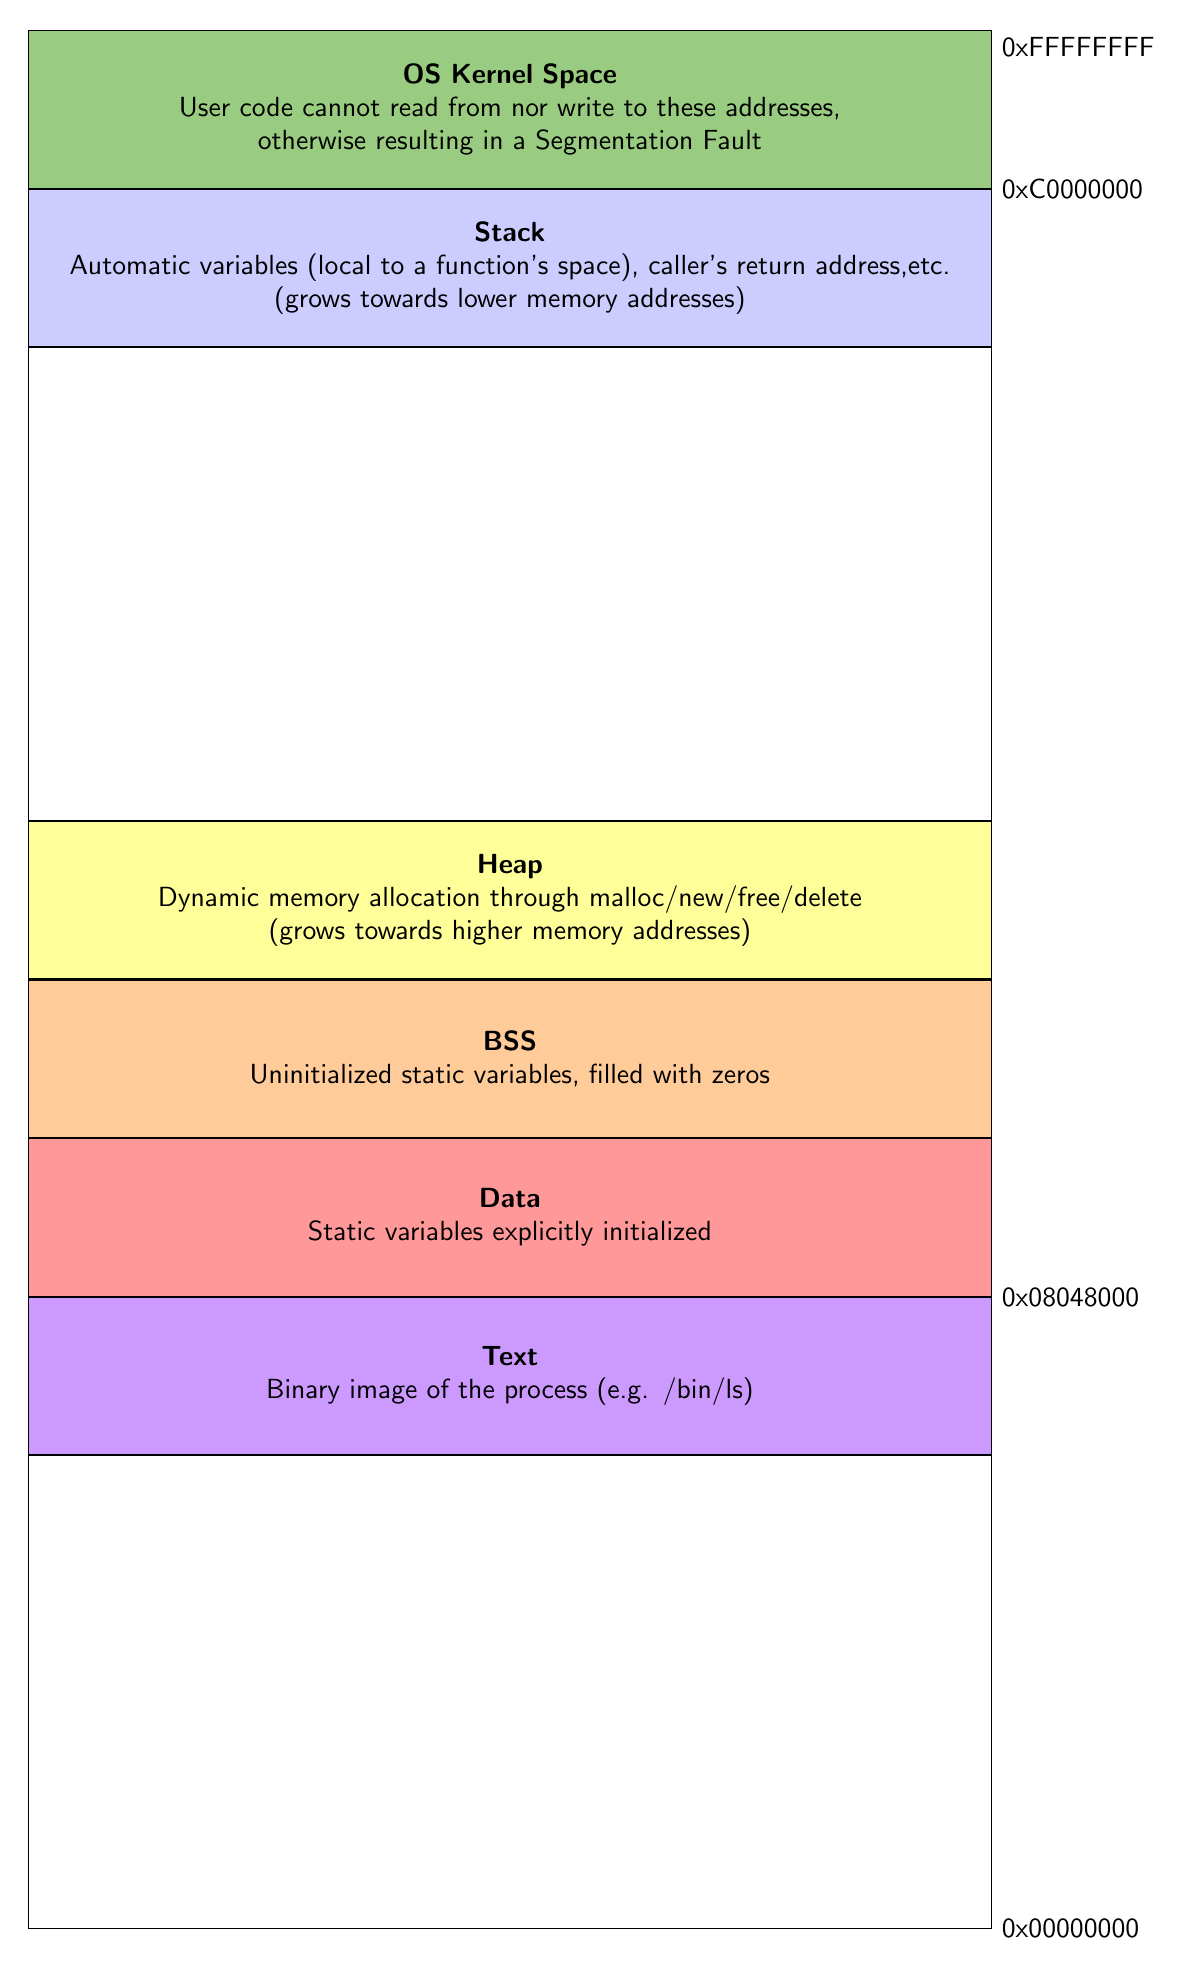
\begin{tikzpicture}[
  node distance=1.5cm and 1cm,
]

% Define colors
\definecolor{osspace-color}{rgb}{0.6, 0.8, 0.5}
\definecolor{stack-color}{rgb}{0.8, 0.8, 1}
\definecolor{heap-color}{rgb}{1, 1, 0.6}
\definecolor{bss-color}{rgb}{1, 0.8, 0.6}
\definecolor{data-color}{rgb}{1, 0.6, 0.6}
\definecolor{text-color}{rgb}{0.8, 0.6, 1}

% Define Node Style
\tikzset{
    every node/.style={font=\sffamily},
    os-kernel-space-style/.style={rectangle, draw, fill=osspace-color, minimum width=12cm, minimum height=2cm, text width=12cm, text centered},
    stack-style/.style={rectangle, draw, fill=stack-color, text width=12cm, text centered, minimum height=2cm, minimum width=12cm},
    blank-style/.style={rectangle, draw, fill=white, text width=12cm, text centered, minimum height=6cm, minimum width=12cm},
    heap-style/.style={rectangle, draw, fill=heap-color, text width=12cm, text centered, minimum height=2cm, minimum width=12cm},
    bss-style/.style={rectangle, draw, fill=bss-color, text width=12cm, text centered, minimum height=2cm, minimum width=12cm},
    data-style/.style={rectangle, draw, fill=data-color, text width=12cm, text centered, minimum height=2cm, minimum width=12cm},
    text-style/.style={rectangle, draw, fill=text-color, text width=12cm, text centered, minimum height=2cm, minimum width=12cm},
    level/.style={anchor=south},
}


% Nodes
\node (os-kernel-space) [os-kernel-space-style] { \textbf{OS Kernel Space} \\ User code cannot read from nor write to these addresses,\\otherwise resulting in a Segmentation Fault};
\node (stack) [stack-style, below=0cm of os-kernel-space] { \textbf{Stack} \\ Automatic variables (local to a function's space), caller's return address,etc.\\(grows towards lower memory addresses)};
\node (blank-after-stack) [blank-style, below=0cm of stack] {};
\node (heap) [heap-style, below=0cm of blank-after-stack] {\textbf{Heap} \\ Dynamic memory allocation through malloc/new/free/delete \\ (grows towards higher memory addresses)};
\node (bss) [bss-style, below=0cm of heap] {\textbf{BSS} \\Uninitialized static variables, filled with zeros};
\node (data) [data-style, below=0cm of bss] {\textbf{Data} \\ Static variables explicitly initialized };
\node (text) [text-style, below=0cm of data] {\textbf{Text} \\ Binary image of the process (e.g. /bin/ls)};
\node (blank-after-text) [blank-style, below=0cm of text] {};

% Add memory addresses
\node[right=of os-kernel-space, yshift=0.8cm,xshift=-1cm] (os-addr) {0xFFFFFFFF};
\node[right=of stack, yshift=1cm,xshift=-1cm] (stack-addr) {0xC0000000};
\node[right=of text,yshift=1cm,xshift=-1cm] (text-addr) {0x08048000};
\node[right=of blank-after-text,yshift=-3cm,xshift=-1cm] (base-addr) {0x00000000};

\end{tikzpicture}

\end{document}
